\chapter{Elastic rod : variational approch}

% #######################################################
\section{Introduction}
% #######################################################

In this section a novel element with 4 degrees of freedom accounting for torsion and bending behaviours is presented. The beam is considered in Kirchhoff’s theory framework, so that it is supposed to be inextensible and its sections are supposed to remain orthogonal to the centreline during deformation. The reduction from the classic 6-DoF model to this 4-DoF model is achieved by an appropriate curve-angle representation based on a relevant curve framing. Energies are then formulated and leads to internal forces and moments acting on the beam. The static equilibrium is deduced from a damped fictitious dynamic with an adapted dynamic relaxation algorithm.

Basile \cite{Bergou2010}

Basile \cite{Bergou2008}
Je
Basile \cite{Audoly2000}

Sina \cite{Nabei2014}


% #######################################################
\section{Kirchhoff rod}
The geometric configuration of the rod is described by its centerline $\vect{x}(s)$ and its cross sections. The centerline is parameterized by its arc-length. Cross sections orientations are followed along the centerline by their material frame $\{\vect{d}_3 (s),\vect{d}_1 (s),\vect{d}_2 (s)\}$ which is an adapted orthonormal moving frame aligned to section’s principal axes of inertia. Here, \guil{adapted} means $\vect{d}_3 (s)=\vect{x}'(s)=\vect{t}(s)$ is aligned to the centerline’s tangent. In the literature, this description is also known as a \emph{Cosserat Curve} \note{[ref]}.

\subsection{Inextensibility}
Note the previous description is only valid for inextensible rods in order to follow material points by their arc-length indifferently in their rest or deformed configuration. As explained in \cite{Audoly2010}, this hypothesis is usually relevant for slender beams. Indeed, in practice, if a slender member faces substantial axial strain the bending behaviour would become negligible due to the important difference between axial and bending stiffness. The length of the rod will be denoted $L$ and the arc-length $s$ will vary (with no loss of generality) in $[0,L]$.

\subsection{Euler-Bernouilli}
Strains are supposed to remain small so that material frame remains orthogonal to the centerline in the deformed configuration. Thus, differentiating the conditions of orthonormality leads to the following differential equations governing the evolution of $\{\vect{d}_3 (s),\vect{d}_1 (s),\vect{d}_2 (s)\}$ along the centerline :
\begin{gather}
	\begin{bmatrix}
		\mathbf{d'_{3}}(s) \\
		\mathbf{d'_{1}}(s) \\
		\mathbf{d'_{2}}(s)
	\end{bmatrix}
	=
	\begin{bmatrix}
		0 & \kappa_{2}(s) & -\kappa_{1}(s) \\
		-\kappa_{2}(s) & 0 & \tau(s) \\
		\kappa_{1}(s) & -\tau(s) & 0
	\end{bmatrix}
	\begin{bmatrix}
		\mathbf{d_{3}}(s) \\
		\mathbf{d_{1}}(s) \\
		\mathbf{d_{2}}(s)
	\end{bmatrix}
\end{gather}

\note{La théorie des poutres est une application de la théorie de l'élasticité isotrope. Pour mener les calculs de résistance des matériaux, on considère les hypothèses suivantes : 

(1) hypothèse de Bernoulli : au cours de la déformation, les sections droites restent perpendiculaires à la courbe moyenne ; 

(2) les sections droites restent planes selon Navier-Bernoulli (pas de gauchissement).

L'hypothèse de Bernoulli permet de négliger le cisaillement dans le cas de la flexion : le risque de rupture est alors dû à l'extension des fibres situées à l'extérieur de la flexion, et la flèche est due au moment fléchissant. Cette hypothèse n'est pas valable pour les poutres courtes car ces dernières sont hors des limites de validité du modèle de poutre, à savoir que la dimension des sections doit être petite devant la longueur de la courbe moyenne. Le cisaillement est pris en compte dans le modèle de Timoshenko et Mindlin.}

\subsection{Darboux vector}
Those equations can be formulated with the \emph{Darboux vector} of the chosen material frame, which represents the rotational velocity of the frame along $\vect{x}(s)$ :
\begin{gather}
	\vect{d}'_{i}(s) = \vect{\Omega}_m(s) \times \vect{d}_i(s)
	\quad,\quad
	\vect{\Omega}_m(s) 
	= 
	\begin{bmatrix}
		\tau(s) \\
		\kappa_{1}(s) \\
		\kappa_{2}(s)
	\end{bmatrix}
\end{gather}
Where $\kappa_1(s)$, $\kappa_2(s)$ and $\tau(s)$ represent respectively the rate of rotation of the material frame around the axis  $\vect{d}_1 (s)$, $\vect{d}_2 (s)$ and $\vect{d}_3 (s)$.

\subsection{Curvatures and twist}
The material curvatures are denoted $\kappa_1(s)$ and $\kappa_2(s)$ and represent the rod’s flexion in the principal planes respectively normal to $\vect{d}_1(s)$ and $\vect{d}_2(s)$ .The material twist is denoted $\tau(s)$ and represents the section’s rate of rotation around $\vect{d}_3(s)$. Those scalar functions measure directly the strain as defined in Kirchhoff’s theory (Figure 4). Recall that the Frenet frame $\{\vect{t}(s),\vect{n}(s),\vect{b}(s)\}$ defines the osculating plane and the total curvature ($\kappa$) of a spatial curve :
\begin{equation}
	\vect{t}'(s) = \kappa(s) \vect{n}(s)
	\quad,\quad
	\kappa(s) = \norm{\vect{t}'(s)}
	\quad,\quad
	\vect{b}(s) = \vect{t}(s) \times \vect{n}(s) = \frac{\vect{t}(s) \times \vect{t}'(s)}{\kappa(s)} 
\end{equation}
To describe the osculating plane in which lies the bending part of the deformation, let’s introduce the \emph{curvature binormal} $\kappa\vect{b}(s) = \vect{t}(s)\times\vect{t}'(s)$, the vector of direction $\vect{b}(s)$ and norm $\kappa(s)$. At each point of arc-length $s$ the osculating plane is normal to $\kappa\vect{b}(s)$.

\subsection{Elastic energy}
Kirrchhoff’s theory assigns an elastic energy to beams according to their strain \cite{Audoly2010}. In this theory, a beam is supposed to be inextensible. Thus the elastic energy ($\mathcal{E}_p$) only accounts for torsion and bending behaviors and is given by :
\begin{equation}
	\mathcal{E}_{p} = 
	\tfrac{1}{2} \int_{0}^{L}EI_1(\kappa_1-\overbar{\kappa_1})^2 + EI_2(\kappa_2-\overbar{\kappa_2})^2 ds
	+ \tfrac{1}{2} \int_{0}^{L} \beta(\tau -{\overbar{\tau}})^2 ds
\end{equation}

Herer, $\overbar{\kappa_1}$, $\overbar{\kappa_2}$ and $\overbar{\tau}$  denote the natural curvature and twist of the rod in the rest position (no stress).

\section{Curve-angle representation}
The previous paragraph has shown how the elastic potential energy of a rod can be computed following both its centerline and its cross sections orientations, which represents a model with 6-DoF : 3 for centerline positions and 3 for cross section orientations.

Following \cite{Bergou2008}, let’s introduce a reduced coordinate formulation of the rod that account for only 4-DoF. This reduction of DoF relies on the concept of zero-twisting frame which gives a reference frame with zero twist along a given centerline. Thus, cross section orientations $\{\vect{d}_3 (s),\vect{d}_1 (s),\vect{d}_2 (s)\}$ can be tracked only by the measure of an angle $\theta$ from this reference frame denoted $\{\vect{d}_3(s),\vect{u}(s),\vect{v}(s)\}$ (Figure 5).

Note that an alternative solution could be to parameterize the global rotations of local material frame and to compute the rotation needed to align two successive frames along the curve’s tangent.

\subsection{Zero-twisting frame}
Zero-twisting frame, also known as Bishop frame, was introduced by Bishop in 1964. Bishop remarked that there was more than one way to frame a curve \cite{Bishop1975}. Indeed, for a given curve, any orthonormal moving frame would satisfy the following differential equations, where $k_1(s)$, $k_2 (s)$ and $\tau(s)$ are scalar functions that define completely the moving frame :
\begin{gather}
	\begin{bmatrix}
		\mathbf{e'_{3}}(s) \\
		\mathbf{e'_{1}}(s) \\
		\mathbf{e'_{2}}(s)
	\end{bmatrix}
=
	\begin{bmatrix}
		0 & k_{2}(s) & -\kappa_{1}(s) \\
		-k_{2}(s) & 0 & \tau(s) \\
		k_{1}(s) & -\tau(s) & 0
	\end{bmatrix}
	\begin{bmatrix}
		\mathbf{e_{3}}(s) \\
		\mathbf{e_{1}}(s) \\
		\mathbf{e_{2}}(s)
	\end{bmatrix}
\end{gather}
For instance, a Frenet frame $\{\vect{t}(s),\vect{n}(s),\vect{b}(s)\}$ is a frame which satisfies $k_1(s)=0$. Note that this frame suffers from major disadvantages : it is undefined where the curvature vanishes and it flips at inflexion points.
A Bishop frame $\{\vect{t}(s),\vect{u}(s),\vect{v}(s)\}$ is a frame which satisfies $\tau(s)=0$. By construction, this frame has no angular velocity (i.e. no twist) around the curve’s tangent ($\vect{u}\cdot\vect{v}' = \vect{u'}\cdot\vect{v}=0$). Its evolution along the curve is described by the corresponding Darboux vector : $\vect{\Omega}_b(s)=\kappa\vect{b}=\vect{t}\times\vect{t'}$. Remark that $\vect{\Omega}_b(s)$ only depends on the centerline and is well defined even when the curvature vanishes.

Thus, by the help of $\vect{\Omega}_b(s)$, it’s possible to transport a given vector $\vect{e}$ along the centerline with no twist : $\vect{e'}=\kappa\vect{b}\times\vect{e}$. This is called \emph{parallel transport}.

\subsection{Bending strains}

Let’s compute the bending strains $\kappa_1$ and $\kappa_2$ regarding the geometric configuration of the rod. Remark that :
\begin{equation}
	\begin{aligned}
	&\kappa\vect{b}\cdot\vect{d}_1 = (\vect{d}_3\times\vect{d}'_3)\cdot\vect{d}_1 = (\vect{d}_1\times\vect{d}_3)\cdot\vect{d}'_3 = -\vect{d}_2\cdot\vect{d}'_3 = \kappa_1 \\
	&\kappa\vect{b}\cdot\vect{d}_2 = (\vect{d}_3\times\vect{d}'_3)\cdot\vect{d}_2 = (\vect{d}_2\times\vect{d}_3)\cdot\vect{d}'_3 = \vect{d}_1\cdot\vect{d}'_3 = \kappa_2	
	\end{aligned}
\end{equation}
That is to say $\kappa\vect{b}$ is orthogonal to $\vect{d}_3$ :
\begin{equation}
	\kappa\vect{b} = \kappa_1\vect{d}_1 +   \kappa_2\vect{d}_2
\end{equation}
Thus, the vector of material curvatures ($\vect{\omega}$) expressed on material frame axes $\{\vect{d}_1(s),\vect{d}_2(s)\}$ is defined as :
\begin{equation}
	\vect{\omega} =
	\begin{bmatrix}
		\kappa_1\\
		\kappa_2\\
	\end{bmatrix} =
	\begin{bmatrix}
		\kappa\vect{b}\cdot\vect{d}_1\\
		\kappa\vect{b}\cdot\vect{d}_2\\
	\end{bmatrix} =
		\begin{bmatrix}
		-\vect{x}''\cdot\vect{d}_2\\
		\vect{x}''\cdot\vect{d}_1\\
	\end{bmatrix}
\end{equation}

\subsection{Torsion strain}
Let’s compute the twist or torsion strain $\tau$ regarding the geometric configuration of the rod. Decomposing the material frame on the bishop frame gives :
\begin{equation}
	\begin{bmatrix}
		\vect{d}_1\\
		\vect{d}_2\\
	\end{bmatrix} =
		\begin{bmatrix}
		\cos{\theta}\;\vect{u} + \sin{\theta}\;\vect{v}\\
		-\sin{\theta}\;\vect{u} + \cos{\theta}\;\vect{v}\\
	\end{bmatrix}
\end{equation}
Thus, the twist can be identified directly as the variation of $\theta$ along the curve :
\begin{equation}
	\tau = \vect{d}'_1 \cdot \vect{d}_2 = (\theta'\vect{d}_2 + \kappa\vect{b}\times\vect{d}_1)\cdot \vect{d}_2 = \theta' + \vect{d}_3\cdot\kappa\vect{b} = \theta'
\end{equation}
Note that the Frenet frame does not lead to a correct evaluation of the twist.

\section{Elastic energy}
Introducing $\vect{\omega}$ and $\theta$, the elastic energy can be rewritten as follow :
\begin{equation}
		\mathcal{E}_{p} = \mathcal{E}_{b} + \mathcal{E}_{t} = 
		\tfrac{1}{2} \int_{0}^{L} (\vect{\omega}-\overbar{\vect{\omega}})^T B (\vect{\omega}-\overbar{\vect{\omega}}) ds
		+ \tfrac{1}{2} \int_{0}^{L} \beta(\theta' -{\overbar{\theta'}})^2 ds
\end{equation}
Where $B$ is the bending stiffness matrix along the principal axes of inertia and $\beta$ is the torsional stiffness :
\begin{equation}
	B = \begin{bmatrix}
			EI_1	&	0\\
			0	&	EI_2\\
		\end{bmatrix}
	\quad,\quad
	\beta = GJ
\end{equation}

\note{
Ici on peut remarquer que l'énergie de torsion est indépendante de $\vect{x}$ et ne dépend donc que de $\theta$.

L'énergie de flexion quant à elle dépend à la fois de $\vect{x}$ et de $\theta$ par l'intermédiaire des vecteurs matériels ($\kappa_1$ et $\kappa_2$ sont les projections de $\kappa\vect{b}$ sur $\vect{d}_1$ et $\vect{d}_2$). Lorsque $EI_1 = EI_2 = EI$, l'énergie de flexion est proportionnelle à la courbure au carré ($EI_1\kappa_1^2 + EI_2\kappa_2^2 = EI\kappa^2$) et par conséquent de dépend plus de $\theta$. En effet, la courbure ($\kappa = ||\kappa\vect{b}|| = ||\vect{x}'\times\vect{x}''||$) ne dépend que de la géométrie de la centerline et pas de l'orientation des sections.
Il n'y a plus de couplage entre la flexion et la torsion et l'énergie totale peut-être minimisée indépendamment en trouvant le minimum de l'énergie de flexion par rapport à la centerline (c'est à dire par rapport à $\vect{x}$ et le minimum de l'énergie de torsion par rapport à l'orientation des sections (c'est à dire par rapport à $\theta$).}

\section{Inextensibility}
Recall that the rod is supposed to be inextensible in Kirchhoff’s theory. Thus, there is no stretching energy associated with an axial strain. However, this constraint will be enforced via a penalty energy, which in practice is somehow very similar as considering an axial stiffness in the beam…

\section{Time-scale assumption}
Following \cite{Bergou2008}, it is relevant to assume that the propagation of twist waves is instantaneous compared to the one of bending waves. Thus, internal forces $\vect{f}^{int}$ and moment $\vect{m}^{int}$ acts on two different timescales in the rod dynamic. Thus on the timescale of action of the force $\vect{f}^{int}$ on the center line, driving the bending waves, the twist waves propagate instantaneously, so that $\forall s \in [0,L],\; \delta\mathcal{E}_{p}/\delta\theta=0$ for the computation of $\vect{f}^{int}$. This assumption may not be enforced, as in \cite{Nabei2014}, but leads to simpler and faster computations.

\section{Gradient}
Internal torsional moments and forces acting on the rod are classically obtained by differentiating the potential energy of the system with respect to $\theta$ and $\vect{x}$. Here, the calculus is a bit tricky as far as the differentiation takes place in function spaces. After a brief reminder on functional derivative, the main results of the calculations of the energy derivatives are given.

\subsection{Derivative of material directors with respect to $\theta$}

Recalling that $\theta$ and $\vect{x}$ are independant variables and that Bishop frame $\{\vect{u},\vect{v}\}$ only depends on $\vect{x}$, the decomposition of material frame directors $\{\vect{d}_1,\vect{d}_2\}$ on Bishop frame leads directly to the following expression for the derivative of the first material director  :
\begin{equation}
			\pdiffof{\theta}{\vect{d}_1}{s}{h_\theta}
	= \frac{d}{d\lambda} \vect{d}_1[\theta + \lambda h_\theta]\Bigr|_{\lambda = 0}
	= \left(-\sin{\theta}\;\vect{u} + \cos{\theta}\;\vect{v}\right) \cdot h_\theta
	= \vect{d}_2\cdot h_\theta \\
\end{equation}
And to the following expression for the derivative of the second material director : 
\begin{equation}
			\pdiffof{\theta}{\vect{d}_2}{s}{h_\theta}
	= \frac{d}{d\lambda} \vect{d}_2[\theta + \lambda h_\theta]\Bigr|_{\lambda = 0}
	= \left(-\cos{\theta}\;\vect{u} - \sin{\theta}\;\vect{v}\right) \cdot h_\theta
	= -\vect{d}_1\cdot h_\theta \\
\end{equation}

\subsection{Derivative of the material curvatures vector with respect to $\theta$}
Regarding the definition of the material curvatures vector and the derivative of material directors with respect to $\theta$, it follows immediately that :
\begin{equation}
			\pdiffof{\theta}{\vect{\omega}}{s}{h_\theta}
	= \frac{d}{d\lambda} \vect{\omega}[\theta + \lambda h_\theta]\Bigr|_{\lambda = 0}
	= \begin{bmatrix}
		\kappa\vect{b}\cdot\vect{d}_2\\
		-\kappa\vect{b}\cdot\vect{d}_1\\
	\end{bmatrix}\cdot h_\theta
	= - \mat{J}\vect{\omega}\cdot h_\theta\\
\end{equation}
Where $\mat{J}$ is the matrix that acts on
two dimensional vectors by counter-clockwise rotation of angle $\frac{\pi}{2}$ : 
\begin{equation}
	\mat{J} = \begin{bmatrix}
			0	&	-1\\
			1	&	0\\
		\end{bmatrix}
\end{equation}

\subsection{Derivative of material directors with respect to $\vect{x}$}

\begin{figure}[t] 
\centering 
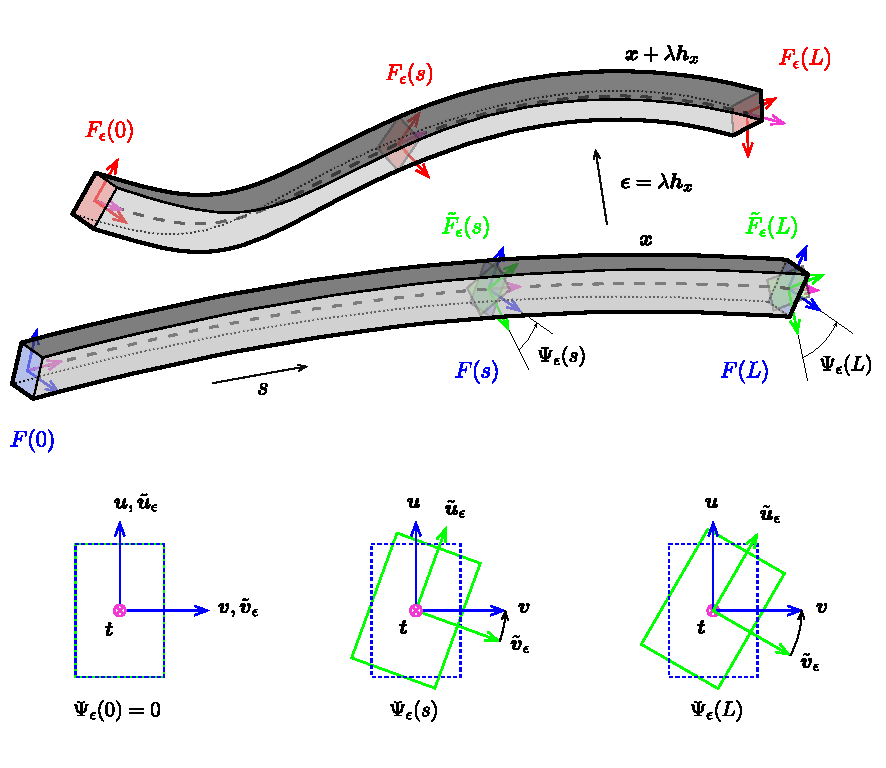
\includegraphics[width=\linewidth]{writhe.pdf} 
\caption{Repères de Frenet attachés à $\gamma$.}
\label{fig:1_1}
\end{figure}

A variation of the centerline would cause a variation in the Bishop frame because parallel transport depends on the centerline itself. As far as $\vect{x}$ and $\theta$ are independent variables, this leads necessarily to a variation of the material frame.

A variation of the centerline would cause a variation in the Bishop frame because parallel transport depends on the centerline itself. As far as $\vect{x}$ and $\theta$ are independent variables, this leads necessarily to a variation of the material frame.

This variation is closely related to the writhe of closed curves. As explained in \cite{Fuller1978} when parallel transporting an adapted frame around a closed curve it might not realigned with itself after one complete loop. This \guil{lack of alignement} is directly measured by the change of writhe which can be computed with Fuller's Formula \cite{Fuller1978}.

One can also see this lack of alignement in terms of rotation. Parallel transport being a propagation of frame from $s = 0$, the cumulated rotation of Bishop frame from the deformed configuration around the initial configuration at arc-length $s$ is the cumulated angle of rotation of $\vect{u}[\vect{x} + \lambda\vect{h}_x]$ around $\vect{d}_3[\vect{x}]$. Recalling the rotation rate of $\vect{u}[\vect{x} + \lambda\vect{h}_x]$ is $\kappa\vect{b}[\vect{x} + \lambda\vect{h}_x]$ by definition of zero-twisting frame, one can write :
\begin{equation}
	\Psi_\epsilon(s) =
	-\int_0^s \kappa\vect{b}[\vect{x} + \lambda\vect{h}_x] \cdot \vect{d}_3[\vect{x}] \,dt
\end{equation}
The calculation of $\kappa\vect{b}[\vect{x} + \lambda\vect{h}_x]$ is straight forward from the curvature binormal definition :
\begin{equation}
	\begin{aligned}
	\kappa\vect{b}[\vect{x} + \lambda\vect{h}_x]
	&= (\vect{x} + \lambda\vect{h}_x)' \times (\vect{x} + \lambda\vect{h}_x)'' \\
	&= \kappa\vect{b}[\vect{x}] + \lambda(\vect{x}'\times\vect{h}''_x + \vect{h}'_x\times\vect{x}'') + \lambda^2(\vect{h}'_x \times \vect{h}''_x) \\
	&= \kappa\vect{b}[\vect{x}] + \lambda(\vect{x}'\times\vect{h}''_x + \vect{h}'_x\times\vect{x}'') + o(\lambda)
	\end{aligned}
\end{equation}
Thus, reminding that $\vect{d}_3[\vect{x}] = \vect{x}'$ and $\kappa\vect{b}[\vect{x}]\cdot\vect{d}_3[\vect{x}] = 0$, and denoting by $\delta_s$ and $H_s$ the Dirac function and the Heaviside step function centered at $s$ :
\begin{equation}
	\begin{aligned}
		\Psi_\epsilon(s) 
		&= -\int_0^s \kappa\vect{b}[\vect{x} + \lambda\vect{h}_x] \cdot \vect{d}_3[\vect{x}] \,dt\\
		&= - \lambda \int_0^s (\vect{x}'\times\vect{h}''_x + \vect{h}'_x\times\vect{x}'') \cdot \vect{x}' \,dt + o(\lambda)\\
		&=  - \lambda \left(\big[\kappa\vect{b}[\vect{x}] \cdot  \vect{h}_x \big]_0^s - \int_0^s \kappa\vect{b}'[\vect{x}] \cdot  \vect{h}_x \,dt\right) + o(\lambda)\\
		&= - \lambda \left(\int_0^s \left(\kappa\vect{b}[\vect{x}]\left(\delta_s-\delta_0\right) - \kappa\vect{b}'[\vect{x}]\right)\cdot  \vect{h}_x \,dt\right) + o(\lambda)\\
		&= - \lambda \left(\int_0^L \left(\kappa\vect{b}[\vect{x}]\left(\delta_s-\delta_0\right) - \kappa\vect{b}'[\vect{x}](1-H_s)\right)\cdot  \vect{h}_x \,dt\right) + o(\lambda)
	\end{aligned}
\end{equation}

\begin{figure}[t] 
\centering 
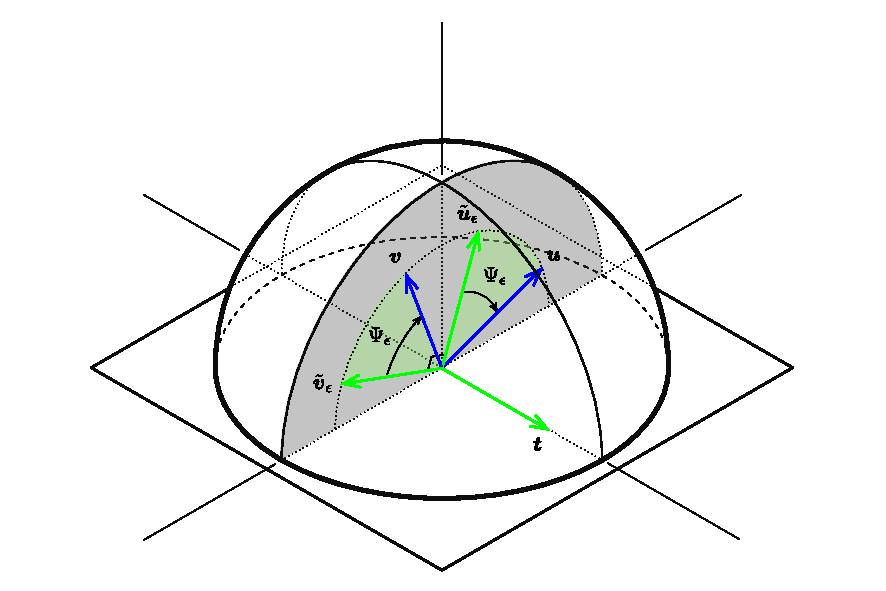
\includegraphics[width=\linewidth]{rotation_A.pdf} 
\caption{Repères de Frenet attachés à $\gamma$.}
\label{fig:1_1}
\end{figure}

This scalar numbers denotes the lack of closure 

To evaluate this change of Bishop frame

\subsubsection{Writhe}
\begin{equation}
	\vect{\tilde{u}}_\epsilon = \cos{\Psi}\;\vect{u} + \sin{\Psi}\;\vect{v}
\end{equation}
\begin{equation}
	\vect{\tilde{v}}_\epsilon = -\sin{\Psi}\;\vect{u} + \cos{\Psi}\;\vect{v}
\end{equation}

\begin{figure}[t] 
\centering 
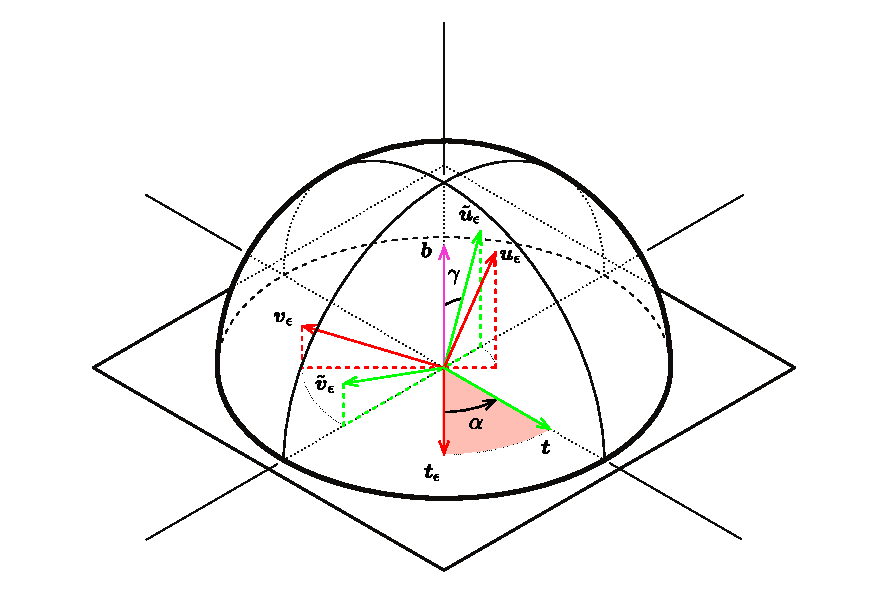
\includegraphics[width=\linewidth]{rotation_B.pdf} 
\caption{$\tilde{F}_\epsilon$ is obtained by parallel tranpsporting $F_\epsilon$ from $\vect{t}_\epsilon$ to $\vect{t}$. This operation could be seen as a rotation around $\vect{t}_\epsilon \times \vect{t}$ of an angle $\alpha$.}
\label{fig:1_1}
\end{figure}

This section is a bit tricky.

$F_\epsilon = \{\vect{t}_\epsilon, \vect{u}_\epsilon,\vect{v}_\epsilon\}$
$\tilde{F}_\epsilon = \{\vect{t}, \vect{\tilde{u}}_\epsilon,\vect{\tilde{v}}_\epsilon\}$
$F = \{\vect{t}, \vect{u},\vect{v}\}$

What we want to achive is to write at arc-length $s$ the Bishop frame in the deformed configuration $\{\vect{t}_\epsilon, \vect{u}_\epsilon,\vect{v}_\epsilon\}$ on the Bishop frame in the reference configuration $\{\vect{t}, \vect{u},\vect{v}\}$.

We first write $\{\vect{t}_\epsilon, \vect{u}_\epsilon,\vect{v}_\epsilon\}$ on the the basis $\{\vect{t}, \vect{\tilde{u}}_\epsilon,\vect{\tilde{v}}_\epsilon\}$. Recall that $\tilde{F}_\epsilon$ is obtained by parallel tranpsporting $F_\epsilon$ from $\vect{t}_\epsilon$ to $\vect{t}$. Denoting :
\begin{equation}
	\vect{b} = \vect{t}_\epsilon \times \vect{t} 
	 = \cos{\gamma}\;\vect{\tilde{u}}_\epsilon + \sin{\gamma}\;\vect{\tilde{v}}_\epsilon
	 = \cos{\gamma}\;\vect{u}_\epsilon + \sin{\gamma}\;\vect{v}_\epsilon
\end{equation}
We have :
\begin{equation}
	\begin{aligned}
	\vect{u}_\epsilon &= \sin{\gamma}\;\vect{b} + \cos{\gamma}\;\big(\sin{\alpha}\;\vect{\tilde{t}}
	+ \cos{\alpha}\;(\cos{\gamma}\;\vect{\tilde{u}_\epsilon} 
	- \sin{\gamma}\;\vect{\tilde{v}_\epsilon})\big) \\
	&=\cos{\gamma}\sin{\alpha}\;\vect{t}
	+ (\cos{\alpha}\cos{\gamma}^2+ \cos{\gamma}^2)\vect{\tilde{u}_\epsilon} 
	+ \sin{\gamma}\cos{\gamma}\;(1-\cos{\alpha})\vect{\tilde{v}_\epsilon} 
	\end{aligned}
\end{equation}
\begin{equation}
	\begin{aligned}
	\vect{v}_\epsilon &= \cos{\gamma}\;\vect{b} + \sin{\gamma}\;\big(-\sin{\alpha}\;\vect{\tilde{t}}
	+ \cos{\alpha}\;(\sin{\gamma}\;\vect{\tilde{u}_\epsilon} 
	- \cos{\gamma}\;\vect{\tilde{v}_\epsilon})\big) \\
	&=-\sin{\gamma}\sin{\alpha}\;\vect{t}
	+ \cos{\gamma}\sin{\gamma}\;(1-\cos{\alpha})\vect{\tilde{u}_\epsilon} 
	+ (\cos{\gamma}^2 + \cos{\alpha}\sin{\gamma}^2)\vect{\tilde{v}_\epsilon} 
	\end{aligned}
\end{equation}

\begin{equation}
	\vect{u}_\epsilon =
	\begin{bmatrix}
		1 & 0 & 0 \\
		0 & \cos{\Psi} & -\sin{\Psi} \\
		0 & \sin{\Psi} & \cos{\Psi} 
	\end{bmatrix}
	\begin{bmatrix}
		\cos{\gamma}\sin{\alpha} \\
		1-2\cos{\gamma}^2\sin{\alpha/2}^2 \\
		2\sin{\gamma}\cos{\gamma}\sin{\alpha/2}^2
	\end{bmatrix}
	=
	\begin{bmatrix}
		\alpha\cos{\gamma}\\
		1 \\
		\Psi
	\end{bmatrix}
	+ o(\lambda)
\end{equation}


\begin{equation}
	\vect{v}_\epsilon =
	\begin{bmatrix}
		1 & 0 & 0 \\
		0 & \cos{\Psi} & -\sin{\Psi} \\
		0 & \sin{\Psi} & \cos{\Psi} 
	\end{bmatrix}
	\begin{bmatrix}
		-\sin{\gamma}\sin{\alpha} \\
		2\sin{\gamma}\cos{\gamma}\sin{\alpha/2}^2 \\
		1-2\sin{\gamma}^2\sin{\alpha/2}^2
	\end{bmatrix}
	=
	\begin{bmatrix}
		-\alpha\sin{\gamma}\\
		-\Psi \\
		1
	\end{bmatrix}
	+ o(\lambda)
\end{equation}

$\tilde{F}_\epsilon(0)$
$\epsilon$

\subsection{Derivative of $\theta$ with respect to $\vect{x}$}


\note{paragraphe entièrment à revoir. Expliquer le cheminement. x fixe bishop et theta fixe d1,d2 par rapport à bishop. x est indépendant de theta. Seul des CL peuvent créer des couplages entre x et theta

Donc les vrais degrés de liberté du problème sont en fait les vecteurs matériels et les positions x. Se reporter à une modélisation du pb dans SO3 comme Spillmann par exemple.

Le calcul des gradients se résume donc à calculer les gradients des vecteurs matériels par rapport à des perturbations infinitésimales en x et theta. Pour theta, c'est facile. Pour kb, c'est facile. Reste la variation par rapport à x, qui est en fait la variation de bishop qu'on explique avec le writhe (défaut de fermeture de bishop sur une boucle fermée) et le transport parallèle.
Le calcul se fait aisément en écrivant la double rotation et en effectuant le DL au premier ordre.

Le reste est quasiment immédiat. Reste la question des CL et des termes aux bords.

Il faut aussi se positionner par rapport à l'article de Basile. Regarder la question applied displacement vs settlement pour imposer une CL.
}

It’s important to notice that the centreline $\vect{x}$ is independent of $\theta$. However, the convers does not hold. Indeed, a variation of the centerline would cause the cross section orientations to be perturbed and thus the potential energy to be modified.

When moving the centerline while conserving section orientation $\{\vect{d}_1,\vect{d}_2\}$,  the angle $\theta$ is modified because the bishop frame is modified. The variation of $\theta$ is thus equal to the opposite of the rotation angle of the bishop frame around $\vect{d}_3$ while the centerline undergoes a variation.

Parallel transport being a propagation of frame from $s = 0$, the variation of $\theta$ at arc-length $s$ is the cumulated angle of rotation of $\vect{u}[\vect{x} + \lambda\vect{h}_x]$ around $\vect{d}_3[\vect{x}]$. Recalling the rotation rate of $\vect{u}[\vect{x} + \lambda\vect{h}_x]$ is $\kappa\vect{b}[\vect{x} + \lambda\vect{h}_x]$ by definition of zero-twisting frame, one can write :
\begin{equation}
	\pdiffof{x}{\theta}{s}{\vect{h}_x} =
	\frac{d}{d\lambda} \int_0^s -\kappa\vect{b}[\vect{x} + \lambda\vect{h}_x] \cdot \vect{d}_3[\vect{x}] \,dt \Bigr|_{\lambda = 0}
\end{equation}
The calculation of $\kappa\vect{b}[\vect{x} + \lambda\vect{h}_x]$ is straight forward from the curvature binormal definition :
\begin{equation}
	\begin{aligned}
	\kappa\vect{b}[\vect{x} + \lambda\vect{h}_x]
	&= (\vect{x} + \lambda\vect{h}_x)' \times (\vect{x} + \lambda\vect{h}_x)'' \\
	&= \kappa\vect{b}[\vect{x}] + \lambda(\vect{x}'\times\vect{h}''_x + \vect{h}'_x\times\vect{x}'') + \lambda^2(\vect{h}'_x \times \vect{h}''_x) \\
	&= \kappa\vect{b}[\vect{x}] + \lambda(\vect{x}'\times\vect{h}''_x + \vect{h}'_x\times\vect{x}'') + o(\lambda)
	\end{aligned}
\end{equation}
Thus, reminding that $\vect{d}_3[\vect{x}] = \vect{x}'$ and denoting by $\delta_s$ and $H_s$ the Dirac function and the Heaviside step function centered at $s$ :
\begin{equation}
	\begin{aligned}
		\pdiffof{x}{\theta}{s}{\vect{h}_x} &= - \int_0^s (\vect{x}'\times\vect{h}''_x + \vect{h}'_x\times\vect{x}'') \cdot \vect{x}' \,dt = \int_0^s \kappa\vect{b}[\vect{x}] \cdot  \vect{h}'_x \,dt\\
		&= \big[\kappa\vect{b}[\vect{x}] \cdot  \vect{h}_x \big]_0^s - \int_0^s \kappa\vect{b}'[\vect{x}] \cdot  \vect{h}_x \,dt \\
		&= \int_0^s \left(\kappa\vect{b}[\vect{x}]\left(\delta_s-\delta_0\right) - \kappa\vect{b}'[\vect{x}]\right)\cdot  \vect{h}_x \,dt \\
		&= \int_0^L \left(\kappa\vect{b}[\vect{x}]\left(\delta_s-\delta_0\right) - \kappa\vect{b}'[\vect{x}](1-H_s)\right)\cdot  \vect{h}_x \,dt \\
		&= \scalar{\frac{\partial\theta}{\partial\vect{x}}(s)}{\vect{h}_x}
	\end{aligned}
\end{equation}
In other words, this means that a variation $\vect{h}_x$ of $\vect{x}$ causes a variation $\int_0^L \frac{\partial\theta}{\partial\vect{x}}(s) \cdot  \vect{h}_x$ of $\theta$ at $s$. Note that this is an integrated quantity, all along the centerline. Finally, the derivative of $\theta$ with respect to $\vect{x}$ is given by :
\begin{equation}
	\frac{\partial\theta}{\partial\vect{x}}(s) = \kappa\vect{b}[\vect{x}]\left(\delta_s-\delta_0\right) - \kappa\vect{b}'[\vect{x}](1-H_s) \in [0,L]^{\mathbb{R}^3}
\end{equation}

Note that the derivative of $\theta$ with respect to $\vect{x}$ can be evaluated by the change of writhe in the curve as suggested in \cite{deVries2005}. This approach is completly equivalent.

\subsection{Derivative of $\vect{\omega}$ with respect to $\vect{x}$}

Let’s express the variation of the material frame after a variation $\lambda \vect{h}_x$ of $\vect{x}$ while $\theta$ remains unchanged. First, remind that material frame remains orthonormal during deformation. Thus, one can write :
\begin{equation}
	\left\{
		\begin{aligned}
			&\vect{d}_1[\vect{x}+\lambda \vect{h}_x] = \vect{d}_1[\vect{x}] + \Delta \Psi \vect{d}_2[\vect{x}] - \Delta \Phi \vect{d}_3[\vect{x}] + o(\lambda)\\
			&\vect{d}_2[\vect{x}+\lambda \vect{h}_x] = \vect{d}_2[\vect{x}] - \Delta \Psi \vect{d}_1[\vect{x}] + \Delta\Gamma \vect{d}_3[\vect{x}] + o(\lambda)
		\end{aligned}
	\right.
\end{equation}
Where $\Delta\Psi$, $\Delta\Gamma$ and $\Delta\Phi$ represent the rotation of $\{\vect{d}_3[\vect{x}+\lambda \vect{h}_x],\vect{d}_1[\vect{x}+\lambda \vect{h}_x],\vect{d}_2[\vect{x}+\lambda \vect{h}_x]\}$, respectively around $\vect{d}_3[\vect{x}]$, $\vect{d}_1[\vect{x}]$, $\vect{d}_2[\vect{x}]$.

Thus, recalling that $\vect{x}''\cdot\vect{d}_3 = 0$ :
\begin{equation}
	\left\{
		\begin{aligned}
			(\vect{x}+\lambda \vect{h}_x)'' \cdot \vect{d}_1[\vect{x}+\lambda \vect{h}_x] = 
			\vect{x}''\cdot\vect{d}_1[\vect{x}] + \lambda(\vect{d}_1[\vect{x}]\cdot\vect{h}''_x + \Delta\Psi \vect{d}_2[\vect{x}]\cdot\vect{x}'') + o(\lambda) \\
			(\vect{x}+\lambda \vect{h}_x)'' \cdot \vect{d}_2[\vect{x}+\lambda \vect{h}_x] =
			\vect{x}''\cdot\vect{d}_2[\vect{x}] + \lambda(\vect{d}_2[\vect{x}]\cdot\vect{h}''_x - \Delta\Psi \vect{d}_1[\vect{x}]\cdot\vect{x}'') + o(\lambda)
		\end{aligned}
		\right.
\end{equation}


% #######################################################
\section{Kinematic}
% #######################################################

Bishop

 $\boldsymbol{x}$ only depends on arc-length along the curve : $\boldsymbol{x}(t)$

Implicit dependence of $\theta$ in $\boldsymbol{x}$ : $\theta(t) \equiv \theta[x](t)$

Implicit dependence of $\boldsymbol{\omega}$ in $\boldsymbol{x}$ and $\theta$ : $\boldsymbol{\omega}(t) \equiv \boldsymbol{\omega}[\boldsymbol{x},\theta](t)$

We denote $\tau$ the twist along the curve : $\tau(t) = \frac{\partial \theta}{\partial t} = \theta'(t)$

We will make the following mathematical assumptions :
\begin{align}
	&\fonction{\boldsymbol{x}}{[0,L]}{\mathbb{R}^3}{t}{\boldsymbol{x}(t)}
	&&\boldsymbol{x} \in \mathcal{C}^{\infty}([0,L]^{\mathbb{R}^3})
	\\ \notag\\
	&\fonction{\theta[\boldsymbol{x}]}{[0,L]}{\mathbb{R}}{t}{\theta[\boldsymbol{x}](t)}
	&&\theta[\boldsymbol{x}] \in \mathcal{C}^{\infty}([0,L]^{\mathbb{R}})
	\\ \notag\\
	&\fonction{\boldsymbol{\omega}[\boldsymbol{x},\theta]}{[0,L]}{\mathbb{R}^2}{t}{\boldsymbol{\omega}[\boldsymbol{x},\theta](t)}
	&&\boldsymbol{\omega}[\boldsymbol{x},\theta] \in \mathcal{C}^{\infty}([0,L]^{\mathbb{R}^2})
\end{align}

The dependence in the arc-length is denoted by the parameter $t \in [0,L]$ by the use of parenthesis $(.)$.
The dependencies in functions are denoted by the use of brackets $[.]$.

When computings energy gradients, it comes to differentiate energies regarding there dependencies in functions $\boldsymbol{x}$ and $\theta$. Thus, we may recall that :
\begin{align}
	&\fonction{\theta}{\mathcal{C}^{\infty}([0,L]^{\mathbb{R}^3})}{\mathcal{C}^{\infty}([0,L]^\mathbb{R})}{\boldsymbol{x}}{\theta[\boldsymbol{x}]}
	&&\theta \in \mathcal{C}^{\infty}
	\\ \notag\\
	&\fonction{\boldsymbol{\omega}}{\mathcal{C}^{\infty}([0,L]^{\mathbb{R}^3}) \times \mathcal{C}^{\infty}([0,L]^{\mathbb{R}})}{\mathcal{C}^{\infty}([0,L]^{\mathbb{R}^2})}{(\boldsymbol{x},\theta)}{\boldsymbol{\omega}[\boldsymbol{x},\theta]}
	&&\boldsymbol{\omega} \in \mathcal{C}^{\infty}
\end{align}





% #######################################################
\section{Energy}
% #######################################################

\begin{align}
\mathcal{E}_p[\boldsymbol{x},\theta] & = \mathcal{E}_{stretch}[\boldsymbol{x}] + \mathcal{E}_{bend}[\boldsymbol{x},\theta] + \mathcal{E}_{twist}[\theta]
\end{align}
\begin{align}
\mathcal{E}_{stretch}[\boldsymbol{x}] & = \tfrac{1}{2} \int_{0}^{L} K_s(\tfrac{\|\boldsymbol{x}'\|}{\|\bar{\boldsymbol{x}}'\|}-1)^2dt \\
\mathcal{E}_{bend}[\boldsymbol{x},\theta] & = \tfrac{1}{2} \int_{0}^{L} (\boldsymbol\omega -\boldsymbol{\bar{\omega}})^T B \, (\boldsymbol\omega -\boldsymbol{\bar{\omega}})dt \\
\mathcal{E}_{twist}[\theta] & = \tfrac{1}{2} \int_{0}^{L} \beta(\theta' -{\bar{\theta'}})^2dt
\end{align}

Energies could be seen as functional, i.e.\ functions that map vectors from a functional vector space to there underlying scalar field $\mathbb{R}$.

\begin{align}
	&\fonctionL{\mathcal{E}_{stretch}}{\mathcal{C}^{\infty}([0,L]^{\mathbb{R}^3})}{\mathbb{R}}{\boldsymbol{x}}{\mathcal{E}_{stretch}[\boldsymbol{x}]}
	\\ \notag\\
	&\fonctionL{\mathcal{E}_{bend}}{\mathcal{C}^{\infty}([0,L]^{\mathbb{R}^3}) \times \mathcal{C}^\infty([0,L]^{\mathbb{R}^3},[0,L]^{\mathbb{R}})}{\mathbb{R}}{(\boldsymbol{x},\theta)}{\mathcal{E}_{bend}[\boldsymbol{x},\theta]}
	\\ \notag\\
	&\fonctionL{\mathcal{E}_{twist}}{\mathcal{C}^\infty([0,L]^{\mathbb{R}^3},[0,L]^{\mathbb{R}})}{\mathbb{R}}{\theta}{\mathcal{E}_{twist}[\theta]}
\end{align}

% #######################################################
\section{Inextensibility}
% #######################################################





% #######################################################
\section{Gradients}
% #######################################################


% --------------------------------------------------------------------------------------------
\subsection{Momentum}
% --------------------------------------------------------------------------------------------

Calcul du moment :
\begin{align}
	\mathcal{M} & = -\frac{d\mathcal{E}_p}{d\theta} =  - \frac{\partial \mathcal{E}_p}{\partial \theta} = - \frac{\partial \mathcal{E}_{bend}}{\partial \theta} - \frac{\partial \mathcal{E}_{twist}}{\partial \theta} \\[0.5em]
\end{align}


\subsubsection{Calcul de $\frac{\partial \mathcal{E}_{twist}}{\partial \theta}$}
% --------------------------------------------------------------------------------------------

\begin{align}
	\mathcal{E}_{twist}[\theta + \lambda h_{\theta}] & = \tfrac{1}{2} \int_{0}^{L} \beta\big((\theta + \lambda h_{\theta})' -{\bar{\theta'}}\big)^2 \,dt \\ 
%   	& = \tfrac{1}{2} \int_{0}^{L} \beta( (\theta'-{\bar{\theta'}})^2 + 2 \lambda (\theta'-{\bar{\theta'}}) h_{\theta}' + \lambda^2 h_{\theta}'^2) \,dt \notag\\
   	& = \mathcal{E}_{twist}[\theta] + \lambda\int_{0}^{L} \beta(\theta'-{\bar{\theta'}}) h_{\theta}' dt +   \lambda^2 \int_{0}^{L} \frac{\beta h_{\theta}'^2}{2} \,dt \notag\\
	& = \mathcal{E}_{twist}[\theta] + \lambda\left[\beta(\theta'-{\bar{\theta'}}) h_{\theta}\right]_0^L - \lambda\int_{0}^{L} \big(\beta(\theta'-{\bar{\theta'}})\big)' h_{\theta}  \,dt + o(\lambda) \notag\\
	& = \mathcal{E}_{twist}[\theta] + \lambda\int_{0}^{L} \big[\beta(\theta'-{\bar{\theta'}})(\delta_L-\delta_0) - \big(\beta(\theta'-{\bar{\theta'}})\big)'\big] h_{\theta}  \,dt + o(\lambda) \notag\\
	& = \mathcal{E}_{twist}[\theta] + \lambda(D_{\mathcal{E}_{twist}} \cdot h_{\theta}) + o(\lambda) \notag
\end{align}

With :
\begin{align}
\frac{\partial \mathcal{E}_{twist}}{\partial \theta} \equiv D_{\mathcal{E}_t} = - \big(\beta(\theta'-{\bar{\theta'}})\big)' + \beta(\theta'-{\bar{\theta'}})(\delta_L-\delta_0) \quad , \quad \frac{\partial \mathcal{E}_{twist}}{\partial \theta} : [0;L] \longrightarrow 	\mathbb{R}
\end{align}



\subsubsection{Calcul de $\frac{\partial \boldsymbol{\omega}}{\partial \theta}$}
% --------------------------------------------------------------------------------------------

On montre par des considérations géométriques que :
\begin{align}
	\boldsymbol{d_1}[\boldsymbol{x}, \theta + \lambda h_{\theta}] & = \boldsymbol{d_1}[\boldsymbol{x}, \theta] + \sin(\lambda h_{\theta})\boldsymbol{d_2}[\boldsymbol{x}, \theta] - (1-\cos(\lambda h_{\theta})\boldsymbol{d_1}[\boldsymbol{x}, \theta] \\
   	& = \boldsymbol{d_1}[\boldsymbol{x}, \theta] + \lambda h_{\theta}\boldsymbol{d_2}[\boldsymbol{x}, \theta] + o(\lambda) \notag
\end{align}
\begin{align}
	\boldsymbol{d_2}[\boldsymbol{x}, \theta + \lambda h_{\theta}] & = \boldsymbol{d_2}[\boldsymbol{x}, \theta] - \sin(\lambda h_{\theta})\boldsymbol{d_1}[\boldsymbol{x}, \theta] - (1-\cos(\lambda h_{\theta})\boldsymbol{d_2}[\boldsymbol{x}, \theta] \\
   	& = \boldsymbol{d_2}[\boldsymbol{x}, \theta] - \lambda h_{\theta}\boldsymbol{d_1}[\boldsymbol{x}, \theta] + o(\lambda) \notag
\end{align}

On en déduit pour le vecteur courbure matérielle :
\begin{align}
	\boldsymbol{\omega}[\boldsymbol{x}, \theta + \lambda h_{\theta}] & = 
	\left[\begin{array}{c}
	\boldsymbol{x}'' \cdot  \boldsymbol{d_1}[\boldsymbol{x}, \theta + \lambda h_{\theta}]\\
	\boldsymbol{x}'' \cdot \boldsymbol{d_2}[\boldsymbol{x}, \theta + \lambda h_{\theta}]\\
	\end{array}\right] \\
	& = \boldsymbol{\omega}[\boldsymbol{x}, \theta] + \lambda 
	\left[\begin{array}{c}
	\boldsymbol{x}'' \cdot  \boldsymbol{d_2}[\boldsymbol{x}, \theta]\\
	- \boldsymbol{x}'' \cdot \boldsymbol{d_1}[\boldsymbol{x}, \theta]\\
	\end{array}\right] \cdot h_{\theta}
	 + o(\lambda)\notag\\
	 & = \boldsymbol{\omega}[\boldsymbol{x}, \theta] + \lambda(D_{\boldsymbol{\omega}} \cdot h_{\theta}) + o(\lambda)\notag
\end{align}

With :
\begin{align}
	&\frac{\partial \boldsymbol{\omega}}{\partial \theta} \equiv D_{\boldsymbol{\omega}} = - R_{\pi/2}\:\boldsymbol{\omega}[\boldsymbol{x}, \theta]
	\quad , \quad R_{\pi/2} = \left[\begin{array}{cc}0 & -1 \\1 & 0\end{array}\right]
	\quad , \quad \frac{\partial \boldsymbol{\omega}}{\partial \theta}  : [0;L] \longrightarrow \mathbb{R}^2
\end{align}


\subsubsection{Calcul de $\frac{\partial \mathcal{E}_{bend}}{\partial \theta}$}
% --------------------------------------------------------------------------------------------

\begin{align}
	\mathcal{E}_{bend}[\boldsymbol{x},\theta + \lambda h_{\theta}]
		& = \tfrac{1}{2} \int_{0}^{L} \big(\boldsymbol{\omega}[\boldsymbol{x}, \theta + \lambda h_{\theta}] - \bar{\boldsymbol{\omega}}[\boldsymbol{x}, \theta]\big)^T B \,  \big(\boldsymbol{\omega}[\boldsymbol{x}, \theta + \lambda h_{\theta}] - \bar{\boldsymbol{\omega}}[\boldsymbol{x}, \theta]\big)dt \notag\\
%	& = \tfrac{1}{2} \int_{0}^{L} \big((\boldsymbol{\omega} - \bar{\boldsymbol{\omega}}) - \lambda R_{\pi/2}\:\boldsymbol{\omega} \cdot h_{\theta} + o(\lambda)\big)^T B \,  \big((\boldsymbol{\omega} - \bar{\boldsymbol{\omega}}) - \lambda R_{\pi/2}\:\boldsymbol{\omega} \cdot h_{\theta} + o(\lambda)\big)dt \notag\\
		& = \mathcal{E}_{bend}[\boldsymbol{x},\theta] - \lambda \int_{0}^{L} \big((\boldsymbol{\omega} - \bar{\boldsymbol{\omega}})^T B R_{\pi/2}\:\boldsymbol{\omega}\big)\cdot h_{\theta} dt + o(\lambda) \notag\\
		& =  \mathcal{E}_{bend}[\boldsymbol{x},\theta] + \lambda(D_{\mathcal{E}_{bend}} \cdot h_{\theta}) + o(\lambda)
\end{align}

With :
\begin{align}
	\frac{\partial \mathcal{E}_{bend}}{\partial \theta} \equiv D_{\mathcal{E}_{bend}} = -(\boldsymbol{\omega} - \bar{\boldsymbol{\omega}})^T B R_{\pi/2}\:\boldsymbol{\omega}
	\quad , \quad \frac{\partial \mathcal{E}_{bend}}{\partial \theta} : [0;L] \longrightarrow \mathbb{R}
\end{align}


\subsubsection{Calcul de $\mathcal{M}$}
% --------------------------------------------------------------------------------------------

Finally:
\begin{align}
\mathcal{M} 	& = -\frac{d\mathcal{E}_p}{d\theta} = -(\boldsymbol{\omega} - \bar{\boldsymbol{\omega}})^T B R_{\pi/2}\:\boldsymbol{\omega} - \big(\beta(\theta'-{\bar{\theta'}})\big)' + \beta(\theta'-{\bar{\theta'}})(\delta_L-\delta_0)
\end{align}

ATTENTION : écrire ici que M est porté par $d_3$

% --------------------------------------------------------------------------------------------
\subsection{Forces}
% --------------------------------------------------------------------------------------------

Calcul des efforts:
\begin{align}
\boldsymbol{\mathcal{F}} & = -\frac{d\mathcal{E}_p}{d\boldsymbol{x}} =  - \frac{\partial \mathcal{E}_p}{\partial \boldsymbol{x}} - \int_{0}^{L} \tfrac{\partial \mathcal{E}_p}{\partial \theta} \tfrac{\partial \theta}{\partial \boldsymbol{x}}
\end{align}


\subsubsection{Calcul de $\frac{\partial \theta}{\partial \boldsymbol{x}}$ par le writh}
% --------------------------------------------------------------------------------------------

\cite{Fuller1978}, \cite{deVries2005},  \cite{Vauquelin2000}, \cite{Berger2009}

On montre ici qu'en un point d'abscisse s, une variation de la centerline de $\lambda \boldsymbol{h_x}$ entraine une variation de $\theta$ intégrée sur la courbe $\Gamma$ de $(\frac{\partial \theta[\boldsymbol{x}](s)}{\partial\boldsymbol{x}} \cdot \lambda \boldsymbol{h_x})$.

$H : t \mapsto \left\{\begin{array}{c}0  , \quad t<0 \\1  , \quad t\geqslant0\end{array}\right.$ est la fonction de Heaviside.

$\delta_{t_0} : t \mapsto \delta(t-t_0)$ est la distribution de dirac centrée en $t_0$.

ATTENTION : ici il y a qqch à expliquer entre $\theta$ et $\psi$ (il y a une question de signe à détailler).

\begin{align}
	\Delta\psi_{\lambda\boldsymbol{h_x}}[\boldsymbol{x}](s) = \psi[\boldsymbol{x} + \lambda\boldsymbol{h_x}](s) - \psi[\boldsymbol{x}](s)
\end{align}

\begin{align}
	\Delta\psi_{\lambda\boldsymbol{h_x}}[\boldsymbol{x}](s) & = \int_{0}^{s} \frac{\boldsymbol{x'} \times (\boldsymbol{x} + \lambda\boldsymbol{h_x})'}{1+ \boldsymbol{x'} \cdot  (\boldsymbol{x} + \lambda\boldsymbol{h_x})'} \cdot \big(\boldsymbol{x''} + (\boldsymbol{x} + \lambda\boldsymbol{h_x})''\big) dt \\
	& = \int_{0}^{s} \frac{\lambda \boldsymbol{x'} \times \boldsymbol{h_x}'}{2(1+ \frac{\lambda \boldsymbol{x'} \cdot \boldsymbol{h_x}'}{2})} \cdot (2\boldsymbol{x''} + \lambda\boldsymbol{h_x}'') dt \notag\\
	& = \int_{0}^{s} \frac{\lambda}{2}(\boldsymbol{x'} \times \boldsymbol{h_x}')\big(1- \frac{\lambda \boldsymbol{x'} \cdot \boldsymbol{h_x}'}{2} + o(\lambda)\big)(2\boldsymbol{x''} + \lambda\boldsymbol{h_x}'') dt \notag\\
	& = \int_{0}^{s} \big(-\boldsymbol{k_b} \cdot \lambda \boldsymbol{h_x'} + \frac{\lambda^2}{2}(\boldsymbol{x'} \times \boldsymbol{h_x}')\cdot\boldsymbol{h_x''}\big)\big(1- \frac{\lambda \boldsymbol{x'} \cdot \boldsymbol{h_x}'}{2} + o(\lambda)\big) dt \notag\\
	& = - \int_{0}^{s} -\boldsymbol{k_b} \cdot \lambda \boldsymbol{h_x'}dt +o(\lambda) \notag\\
	& = \big[-\boldsymbol{k_b} \cdot \lambda \boldsymbol{h_x}\big]_{0}^{s} + \int_{0}^{s} \boldsymbol{k_b'} \cdot \lambda \boldsymbol{h_x}dt +o(\lambda) \notag\\
	& = \int_{0}^{L} \big((1-H)\boldsymbol{k_b'} - (\delta_s - \delta_0)\boldsymbol{k_b}\big)\cdot\lambda \boldsymbol{h_x}dt +o(\lambda) \notag\\
	& = \lambda(\boldsymbol{D_{\psi}}(s)\cdot\boldsymbol{h_x}) + o(\lambda)\notag
\end{align}

With :
\begin{align}
	\frac{\partial \theta}{\partial \boldsymbol{x}}(s) \equiv -\boldsymbol{D_{\psi}}(s) = (\delta_s - \delta_0)\boldsymbol{k_b} - (1-H)\boldsymbol{k_b'}
	\quad , \quad \frac{\partial \theta}{\partial \boldsymbol{x}}(s) : [0;L] \longrightarrow \mathbb{R}^3
\end{align}



\subsubsection{Calcul de $\frac{\partial \boldsymbol{\omega}}{\partial \boldsymbol{x}}$}
% --------------------------------------------------------------------------------------------

Quand $\boldsymbol{x}$ varie de $\lambda\boldsymbol{h_x}$, le repère materiel est tourné de sorte que, en décomposant sur le repère de base :
\begin{align}
	\boldsymbol{d_1}[\boldsymbol{x}+\lambda\boldsymbol{h_x}, \theta] & = \boldsymbol{d_1}[\boldsymbol{x}, \theta] + \Delta\psi_{\lambda\boldsymbol{h_x}}[\boldsymbol{x}]\boldsymbol{d_2}[\boldsymbol{x}, \theta] + \Delta\phi_{\lambda\boldsymbol{h_x}}[\boldsymbol{x}]\boldsymbol{d_3}[\boldsymbol{x}, \theta] + o(\lambda)\\
	\boldsymbol{d_2}[\boldsymbol{x}+\lambda\boldsymbol{h_x}, \theta] & = \boldsymbol{d_2}[\boldsymbol{x}, \theta] - \Delta\psi_{\lambda\boldsymbol{h_x}}[\boldsymbol{x}]\boldsymbol{d_1}[\boldsymbol{x}, \theta] - \Delta\phi_{\lambda\boldsymbol{h_x}}[\boldsymbol{x}]\boldsymbol{d_3}[\boldsymbol{x}, \theta] + o(\lambda)
\end{align}
On montre aisément que la contribution en $\Delta\psi$ autour de $\boldsymbol{d_1}$ et $\boldsymbol{d_2}$ est d'un ordre supérieur à celle autour de $\boldsymbol{d_3} = \boldsymbol{x}'$ (ce qui se comprend bien dans le cas d'une variation en hélice).

Par propriété d'orthogonalité des vecteurs du repère mobile (cf § sur le curve framing) on montre que :
\begin{align}
	\boldsymbol{d_1}\cdot\boldsymbol{d_3} = 0 &\Rightarrow \boldsymbol{d_1}[\boldsymbol{x}+\lambda\boldsymbol{h_x}, \theta] \cdot (\boldsymbol{x}+\lambda\boldsymbol{h_x})' = 0\\
	&\Rightarrow \Delta\phi_{\lambda\boldsymbol{h_x}}[\boldsymbol{x}] = \boldsymbol{d_1}[\boldsymbol{x}+\lambda\boldsymbol{h_x}, \theta] \cdot \boldsymbol{x}' = \lambda(-\boldsymbol{d_1}[\boldsymbol{x}, \theta] \cdot \boldsymbol{h_x}') + o(\lambda) \notag
\end{align}
\begin{align}
	\boldsymbol{d_2}\cdot\boldsymbol{d_3} = 0 &\Rightarrow \boldsymbol{d_1}[\boldsymbol{x}+\lambda\boldsymbol{h_x}, \theta] \cdot (\boldsymbol{x}+\lambda\boldsymbol{h_x})' = 0\\
	&\Rightarrow \Delta\phi_{\lambda\boldsymbol{h_x}}[\boldsymbol{x}] = \boldsymbol{d_2}[\boldsymbol{x}+\lambda\boldsymbol{h_x}, \theta] \cdot \boldsymbol{x}' = \lambda(-\boldsymbol{d_2}[\boldsymbol{x}, \theta] \cdot \boldsymbol{h_x}') + o(\lambda) \notag
\end{align}

On en déduit le calcul de la variation de $\boldsymbol{\omega}$ pour une vairation de la centerline de $\lambda \boldsymbol{h_x}$ qui vaut :
\begin{align}
	\boldsymbol{\omega}[\boldsymbol{x}+\lambda \boldsymbol{h_x},\theta]
	& =
	\left[\begin{array}{c}
	(\boldsymbol{x}+\lambda \boldsymbol{h_x})'' \cdot  \boldsymbol{d_1}[\boldsymbol{x}+\lambda \boldsymbol{h_x},\theta]\\
	(\boldsymbol{x}+\lambda \boldsymbol{h_x})'' \cdot \boldsymbol{d_2}[\boldsymbol{x}+\lambda \boldsymbol{h_x},\theta]\\
	\end{array}\right] \notag\\
	& = 
	\left[\begin{array}{c}
	(\boldsymbol{x}+\lambda \boldsymbol{h_x})'' \cdot ( 	\boldsymbol{d_1}[\boldsymbol{x}] 
												+ (-\lambda\frac{\partial \theta}{\partial \boldsymbol{x}}(s) \cdot \boldsymbol{h_x} + o(\lambda))\boldsymbol{d_2}[\boldsymbol{x}]
												- (\lambda \boldsymbol{d_1[\boldsymbol{x}]}\cdot\boldsymbol{h_x} + o(\lambda)) \cdot \boldsymbol{x}''
											)\\
	(\boldsymbol{x}+\lambda \boldsymbol{h_x})'' \cdot ( 	\boldsymbol{d_2}[\boldsymbol{x}] 
												- (-\lambda\frac{\partial \theta}{\partial \boldsymbol{x}}(s) \cdot \boldsymbol{h_x} + o(\lambda))\boldsymbol{d_1}[\boldsymbol{x}]
												- (\lambda \boldsymbol{d_2[\boldsymbol{x}]}\cdot\boldsymbol{h_x} + o(\lambda)) \cdot \boldsymbol{x}''
											)\\
	\end{array}\right] \notag\\
	  \begin{split}
      		& = \boldsymbol{\omega}[\boldsymbol{x},\theta] +
        			\lambda
        			\left[\begin{array}{c}
        			\boldsymbol{d_1}[\boldsymbol{x},\theta]^T \\
        			\boldsymbol{d_2}[\boldsymbol{x},\theta]^T
        			\end{array}\right] \cdot \boldsymbol{h_x}'' 
        			 -
        			\big(\lambda\frac{\partial \theta}{\partial \boldsymbol{x}}(s) \cdot \boldsymbol{h_x}\big)
        			\left[\begin{array}{c}
        			\boldsymbol{d_2}[\boldsymbol{x},\theta]\cdot \boldsymbol{x}''\\
        			-\boldsymbol{d_1}[\boldsymbol{x},\theta]\cdot \boldsymbol{x}''\\
        			\end{array}\right] \\
        		& \hspace{5cm}+ \lambda(\boldsymbol{x}'' \cdot \boldsymbol{x}')
        		\left[\begin{array}{c}
        		\boldsymbol{d_1}[\boldsymbol{x},\theta]\cdot \boldsymbol{h_x}'\\
        		\boldsymbol{d_2}[\boldsymbol{x},\theta]\cdot \boldsymbol{h_x}''\\
        		\end{array}\right]
        		 + o(\lambda)
 	 \end{split} \notag
\end{align}


\begin{align}
	\boldsymbol{\omega}[\boldsymbol{x}+\lambda \boldsymbol{h_x},\theta] & = 
	\left[\begin{array}{c}
		(\boldsymbol{x}+\lambda \boldsymbol{h_x})'' \cdot  \boldsymbol{d_1}[\boldsymbol{x}+\lambda \boldsymbol{h_x},\theta]\\
		(\boldsymbol{x}+\lambda \boldsymbol{h_x})'' \cdot \boldsymbol{d_2}[\boldsymbol{x}+\lambda \boldsymbol{h_x},\theta]\\
	\end{array}\right] && POUET &&& POUET\notag\\
& = 
\left[\begin{array}{c}
	(\boldsymbol{x}+\lambda \boldsymbol{h_x})'' \cdot ( 	\boldsymbol{d_1}[\boldsymbol{x}] 
												+ (-\lambda\frac{\partial \theta}{\partial \boldsymbol{x}}(s) \cdot \boldsymbol{h_x} + o(\lambda))\boldsymbol{d_2}[\boldsymbol{x}]
											)\\
	(\boldsymbol{x}+\lambda \boldsymbol{h_x})'' \cdot ( 	\boldsymbol{d_2}[\boldsymbol{x}] 
												- (-\lambda\frac{\partial \theta}{\partial \boldsymbol{x}}(s) \cdot \boldsymbol{h_x} + o(\lambda))\boldsymbol{d_1}[\boldsymbol{x}]
											)\\
	\end{array}\right] && POUET &&& POUET\notag\\
& \quad- 
\left[\begin{array}{c}
												- (\lambda \boldsymbol{d_1[\boldsymbol{x}]}\cdot\boldsymbol{h_x} + o(\lambda)) \cdot \boldsymbol{x}''
											)\\
												- (\lambda \boldsymbol{d_2[\boldsymbol{x}]}\cdot\boldsymbol{h_x} + o(\lambda)) \cdot \boldsymbol{x}''
											)\\
	\end{array}\right] && POUET &&& POUET\notag\\
\end{align}



\begin{align}
  g + h & = i \\
  \begin{split}
      a & = b + c - d \\
        & \quad + e - f
  \end{split} \\
\end{align}

\begin{equation}\label{e:barwq}\begin{split}
H_c&=\frac{1}{2n} \sum^n_{l=0}(-1)^{l}(n-{l})^{p-2}
\sum_{l _1+\dots+ l _p=l}\prod^p_{i=1} \binom{n_i}{l _i}\\ 
&\quad\cdot[(n-l )-(n_i-l _i)]^{n_i-l _i}\cdot
\Bigl[(n-l )^2-\sum^p_{j=1}(n_i-l _i)^2\Bigr].
\end{split}\end{equation}

	\begin{align}
        		\boldsymbol{\omega}[\boldsymbol{x},\theta] +
        		\lambda
        		\left[\begin{array}{c}
        		\boldsymbol{d_1}[\boldsymbol{x}]^T \\
        		\boldsymbol{d_2}[\boldsymbol{x}]^T
        		\end{array}\right] \cdot \boldsymbol{h_x}'' 
        		& -
        		\big(\lambda\frac{\partial \theta}{\partial \boldsymbol{x}}(s) \cdot \boldsymbol{h_x}\big)
        		\left[\begin{array}{c}
        		\boldsymbol{d_2}[\boldsymbol{x},\theta]\cdot \boldsymbol{x}''\\
        		-\boldsymbol{d_1}[\boldsymbol{x},\theta]\cdot \boldsymbol{x}''\\
        		\end{array}\right] \\
        		& - 
        		\lambda(\boldsymbol{x}'' \cdot \boldsymbol{x}')
        		\left[\begin{array}{c}
        		\boldsymbol{d_1}[\boldsymbol{x},\theta]\cdot \boldsymbol{h_x}'\\
        		\boldsymbol{d_2}[\boldsymbol{x},\theta]\cdot \boldsymbol{h_x}''\\
        		\end{array}\right] \\
        		& + o(\lambda)
	\end{align}

% #######################################################
\section{Discretization}
% #######################################################




% #######################################################
\section{Connection}
% #######################################################


\bibliographystyle{alpha}
\bibliography{../bibliography}